\documentclass[aspectratio=169,12pt]{beamer}

% ===== PACKAGES =====
\usepackage[utf8]{inputenc}
\usepackage[T1]{fontenc}
\usepackage{lmodern}
\usepackage{tikz}
\usetikzlibrary{shapes,arrows.meta,positioning,calc,backgrounds,fit}
\usepackage{fontawesome5}
\usepackage{booktabs}
\usepackage{array}
\usepackage{graphicx}
\usepackage{multicol}

% ===== COLORS =====
\definecolor{navy}{HTML}{1E3A5F}
\definecolor{gold}{HTML}{C9A742}
\definecolor{lightgold}{HTML}{FDF6E3}
\definecolor{darktext}{HTML}{2C2C2C}
\definecolor{offwhite}{HTML}{F5F3EE}
\definecolor{softgray}{HTML}{8A8A8A}
\definecolor{warmred}{HTML}{A0332E}
\definecolor{teal}{HTML}{1B6B6D}
\definecolor{deepnavy}{HTML}{0D2E40}
\definecolor{lightblue}{HTML}{E8EFF7}

% ===== BEAMER THEME =====
\usetheme{default}
\usecolortheme{default}
\setbeamercolor{background canvas}{bg=white}
\setbeamercolor{normal text}{fg=darktext}
\setbeamercolor{frametitle}{fg=navy,bg=}
\setbeamercolor{title}{fg=white}
\setbeamercolor{subtitle}{fg=gold}
\setbeamercolor{author}{fg=white}
\setbeamercolor{institute}{fg=softgray}
\setbeamercolor{date}{fg=softgray}

\setbeamerfont{frametitle}{series=\bfseries,size=\Large,family=\rmfamily}
\setbeamerfont{title}{series=\bfseries,size=\huge,family=\rmfamily}
\setbeamerfont{subtitle}{series=\mdseries,size=\large,family=\rmfamily}
\setbeamerfont{framesubtitle}{series=\mdseries,size=\normalsize}

% Remove navigation symbols
\setbeamertemplate{navigation symbols}{}

% ===== PERSISTENT FOOTER ON ALL SLIDES (including plain) =====
% This uses TikZ overlay so it appears on EVERY frame without exception
\addtobeamertemplate{background}{}{%
    \begin{tikzpicture}[remember picture, overlay]
        \node[anchor=south west, inner sep=0pt, text width=0.45\paperwidth]
            at ([xshift=0.8em, yshift=0.4em]current page.south west)
            {\tiny\color{softgray} \textsc{ICF Word Study} --- Moscow Good News Church};
        \node[anchor=south, inner sep=0pt]
            at ([yshift=0.4em]current page.south)
            {\tiny\color{softgray}\textit{$\sim$~Roger Nick Anaedevha}};
        \node[anchor=south east, inner sep=0pt]
            at ([xshift=-0.8em, yshift=0.4em]current page.south east)
            {\tiny\color{softgray} \insertframenumber\,/\,\inserttotalframenumber};
    \end{tikzpicture}%
}

% Suppress default footline (we use TikZ overlay above instead)
\setbeamertemplate{footline}{}

% Custom frametitle with gold underline
\setbeamertemplate{frametitle}{%
    \vspace{0.3cm}%
    \insertframetitle%
    \vspace{2pt}%
    {\color{gold}\rule{3cm}{1.5pt}}%
    \par%
    \vspace{0.1cm}%
}

% Itemize styling
\setbeamertemplate{itemize items}[circle]
\setbeamercolor{itemize item}{fg=gold}
\setbeamercolor{itemize subitem}{fg=teal}

% Block styling
\setbeamercolor{block title}{bg=navy,fg=white}
\setbeamercolor{block body}{bg=lightgold,fg=darktext}
\setbeamercolor{block title alerted}{bg=warmred,fg=white}
\setbeamercolor{block body alerted}{bg=lightgold,fg=darktext}
\setbeamercolor{block title example}{bg=teal,fg=white}
\setbeamercolor{block body example}{bg=lightblue,fg=darktext}

% ===== CUSTOM COMMANDS =====
\newcommand{\goldline}{\par\vspace{4pt}{\color{gold}\rule{2.5cm}{1.2pt}}\par\vspace{4pt}}
\newcommand{\scriptref}[1]{{\small\color{teal}\faIcon{bible}~\textit{#1}}}

% ===== DARK-SLIDE FOOTER (gold text on navy backgrounds) =====
% Redefine for dark slides so footer text is visible
\newcommand{\darkfooteroverlay}{%
    \begin{tikzpicture}[remember picture, overlay]
        \node[anchor=south west, inner sep=0pt, text width=0.45\paperwidth]
            at ([xshift=0.8em, yshift=0.4em]current page.south west)
            {\tiny\color{gold!70!white} \textsc{ICF Word Study} --- Moscow Good News Church};
        \node[anchor=south, inner sep=0pt]
            at ([yshift=0.4em]current page.south)
            {\tiny\color{gold!70!white}\textit{$\sim$~Roger Nick Anaedevha}};
        \node[anchor=south east, inner sep=0pt]
            at ([xshift=-0.8em, yshift=0.4em]current page.south east)
            {\tiny\color{gold!70!white} \insertframenumber\,/\,\inserttotalframenumber};
    \end{tikzpicture}%
}

% ===== DOCUMENT INFO =====
\title{Being Led by the\\Written Word (\textit{Logos})}
\subtitle{( Logos --- $\lambda\acute{o}\gamma o\varsigma$ )}
\author{$\sim$~Roger Nick Anaedevha}
\institute{\textsc{ICF Word Study}\\Moscow Good News Church}
\date{March 20, 2026}

% ====================================================================
\begin{document}

% ============================================================
% SLIDE 1 — TITLE
% ============================================================
{
\setbeamercolor{background canvas}{bg=navy}
\begin{frame}[plain]
\darkfooteroverlay
\vfill
\begin{center}

{\large\bfseries\color{gold}\textsc{ICF Word Study}}\\[2pt]
{\small\color{softgray} Moscow Good News Church}

\vspace{0.5cm}

{\huge\bfseries\color{white} Being Led by the\\[4pt] Written Word (\textit{Logos})}

\vspace{0.2cm}
{\color{gold}\rule{6cm}{1.5pt}}
\vspace{0.2cm}

{\large\color{white} Bible Study Series --- Part 1 of 2}\\[6pt]
{\normalsize\color{gold} Psalm 119:105~~$\cdot$~~2 Timothy 3:16--17}

\vspace{0.5cm}
{\normalsize\color{white}\textit{$\sim$~Roger Nick Anaedevha}}

\vspace{0.3cm}
{\small\color{softgray} March 20, 2026}
\end{center}
\vfill
\end{frame}
}

% ============================================================
% SLIDE 2 — SERIES OVERVIEW
% ============================================================
\begin{frame}{Series Overview}

\begin{columns}[T]
\begin{column}{0.48\textwidth}

\begin{tikzpicture}
\node[fill=navy, rounded corners=4pt, minimum width=\textwidth, minimum height=3.8cm, anchor=north west, text width=0.9\textwidth] (box) at (0,0) {};
\node[fill=gold, rounded corners=2pt, minimum width=\textwidth, minimum height=0.5cm, anchor=north west] at (0,0) {\footnotesize\bfseries\color{navy} PART 1 --- TODAY};
\node[anchor=north west, text width=0.85\textwidth] at (0.15,-0.7) {
    {\color{white}\bfseries\rmfamily Being Led by the\\Written Word (Logos)}\\[4pt]
    {\color{gold}\scriptsize Psalm 119:105 / 2 Tim 3:16--17}\\[6pt]
    {\color{white}\scriptsize\itshape The Bible as our foundational\\lamp and God-breathed authority.}
};
\end{tikzpicture}
\end{column}
\begin{column}{0.48\textwidth}
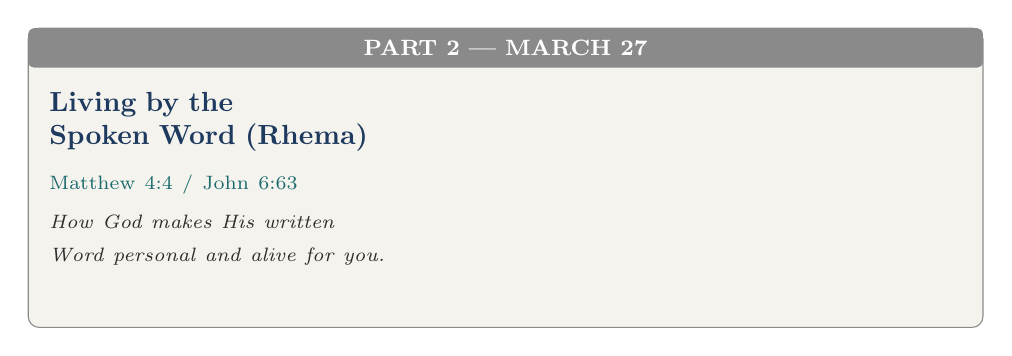
\begin{tikzpicture}
\node[fill=offwhite, draw=softgray, rounded corners=4pt, minimum width=\textwidth, minimum height=3.8cm, anchor=north west, text width=0.9\textwidth] (box) at (0,0) {};
\node[fill=softgray, rounded corners=2pt, minimum width=\textwidth, minimum height=0.5cm, anchor=north west] at (0,0) {\footnotesize\bfseries\color{white} PART 2 --- MARCH 27};
\node[anchor=north west, text width=0.85\textwidth] at (0.15,-0.7) {
    {\color{navy}\bfseries\rmfamily Living by the\\Spoken Word (Rhema)}\\[4pt]
    {\color{teal}\scriptsize Matthew 4:4 / John 6:63}\\[6pt]
    {\color{darktext}\scriptsize\itshape How God makes His written\\Word personal and alive for you.}
};
\end{tikzpicture}
\end{column}
\end{columns}

\vspace{0.4cm}

\begin{tikzpicture}
\node[fill=lightgold, rounded corners=3pt, minimum width=\textwidth, inner sep=6pt] {
    \small\bfseries\color{navy} KEY PRINCIPLE: Logos must come before Rhema --- the written Word is the foundation.
};
\end{tikzpicture}

\end{frame}

% ============================================================
% SLIDE 3 — WHAT IS LOGOS?
% ============================================================
\begin{frame}{What Is Logos?}

\begin{columns}[T]
\begin{column}{0.48\textwidth}

\vspace{-0.2cm}

% Meaning 1
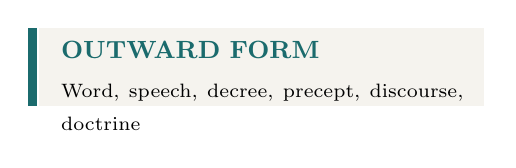
\begin{tikzpicture}
\fill[teal] (0,0) rectangle (0.12,1);
\fill[offwhite] (0.15,0) rectangle (5.8,1);
\node[anchor=north west, text width=5.3cm] at (0.3,0.95) {
    {\small\bfseries\color{teal} OUTWARD FORM}\\[2pt]
    {\scriptsize Word, speech, decree, precept, discourse, doctrine}
};
\end{tikzpicture}

\vspace{0.15cm}

% Meaning 2
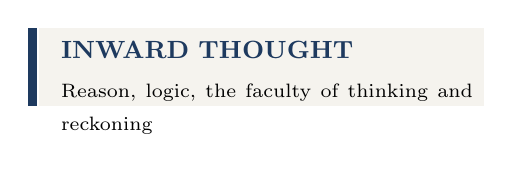
\begin{tikzpicture}
\fill[navy] (0,0) rectangle (0.12,1);
\fill[offwhite] (0.15,0) rectangle (5.8,1);
\node[anchor=north west, text width=5.3cm] at (0.3,0.95) {
    {\small\bfseries\color{navy} INWARD THOUGHT}\\[2pt]
    {\scriptsize Reason, logic, the faculty of thinking and reckoning}
};
\end{tikzpicture}

\vspace{0.15cm}

% Meaning 3
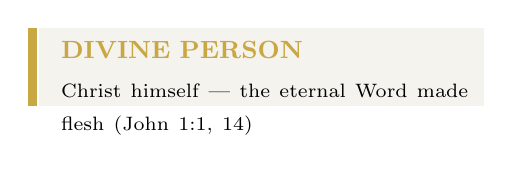
\begin{tikzpicture}
\fill[gold] (0,0) rectangle (0.12,1);
\fill[offwhite] (0.15,0) rectangle (5.8,1);
\node[anchor=north west, text width=5.3cm] at (0.3,0.95) {
    {\small\bfseries\color{gold} DIVINE PERSON}\\[2pt]
    {\scriptsize Christ himself --- the eternal Word made flesh (John 1:1, 14)}
};
\end{tikzpicture}

\end{column}
\begin{column}{0.48\textwidth}

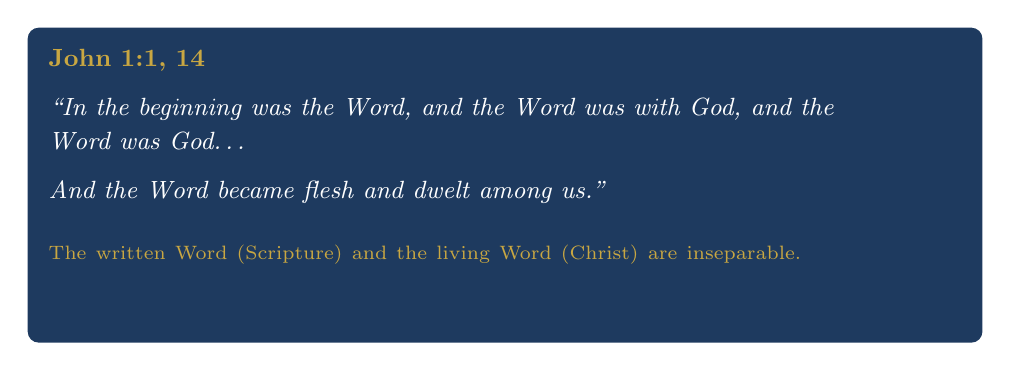
\begin{tikzpicture}
\node[fill=navy, rounded corners=4pt, minimum width=\textwidth, minimum height=4cm, anchor=north west, text width=0.9\textwidth] (box) at (0,0) {};
\node[anchor=north west, text width=0.85\textwidth] at (0.15,-0.15) {
    {\small\bfseries\color{gold} John 1:1, 14}\\[6pt]
    {\small\color{white}\itshape\rmfamily ``In the beginning was the Word, and the Word was with God, and the Word was God\ldots}\\[6pt]
    {\small\color{white}\itshape\rmfamily And the Word became flesh and dwelt among us.''}\\[10pt]
    {\scriptsize\color{gold} The written Word (Scripture) and the living Word (Christ) are inseparable.}
};
\end{tikzpicture}

\end{column}
\end{columns}

\end{frame}

% ============================================================
% SLIDE 4 — PSALM 119:105
% ============================================================
\begin{frame}{Psalm 119:105 --- Lamp \& Light}

\begin{center}
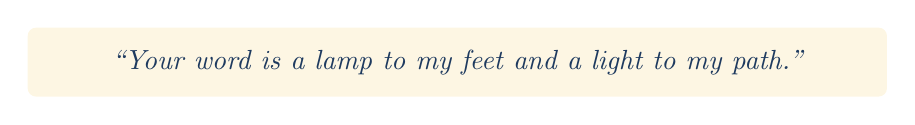
\begin{tikzpicture}
\node[fill=lightgold, rounded corners=3pt, minimum width=0.9\textwidth, inner sep=8pt] {
    \rmfamily\itshape\color{navy} ``Your word is a lamp to my feet and a light to my path.''
};
\end{tikzpicture}
\end{center}

\vspace{0.2cm}

\begin{columns}[T]
\begin{column}{0.48\textwidth}
\begin{block}{\faIcon{fire}~~NER --- Lamp to My Feet}
\vspace{2pt}
\textbf{\color{teal}Immediate Guidance}\\[4pt]
{\small Small handheld oil lamp --- carried by travelers at night in ancient towns without street lamps.}\\[6pt]
{\small\bfseries\color{navy} $\rightarrow$ Present decisions, current problems, the very next step you need to take.}
\end{block}
\end{column}
\begin{column}{0.48\textwidth}
\begin{exampleblock}{\faIcon{sun}~~OR --- Light to My Path}
\vspace{2pt}
\textbf{\color{gold}Broader Direction}\\[4pt]
{\small Wider illumination --- seeing the trajectory of your journey and God's purposes for life.}\\[6pt]
{\small\bfseries\color{navy} $\rightarrow$ Life direction, moral vision, long-range spiritual discernment.}
\end{exampleblock}
\end{column}
\end{columns}

\end{frame}

% ============================================================
% SLIDE 5 — 2 TIMOTHY 3:16-17 (THEOPNEUSTOS)
% ============================================================
\begin{frame}{2 Timothy 3:16--17 --- God-Breathed}

\begin{columns}[T]
\begin{column}{0.48\textwidth}

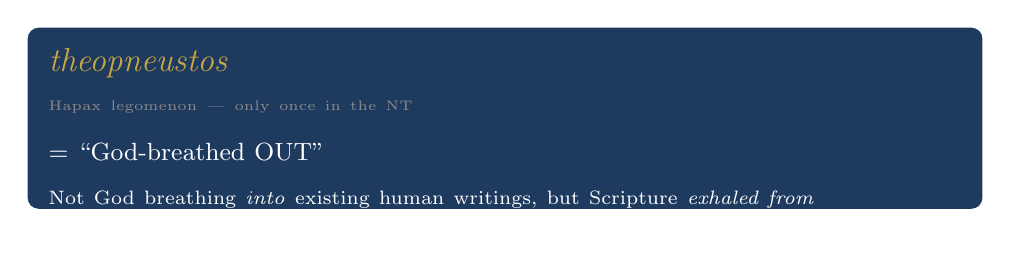
\begin{tikzpicture}
\node[fill=navy, rounded corners=4pt, minimum width=\textwidth, minimum height=2.3cm, anchor=north west, text width=0.9\textwidth] (box) at (0,0) {};
\node[anchor=north west, text width=0.85\textwidth] at (0.15,-0.15) {
    {\large\color{gold}\itshape\rmfamily theopneustos}\\[2pt]
    {\tiny\color{softgray} Hapax legomenon --- only once in the NT}\\[6pt]
    {\small\color{white} = ``God-breathed OUT''}\\[4pt]
    {\scriptsize\color{white} Not God breathing \textit{into} existing human writings, but Scripture \textit{exhaled from God himself}.}
};
\end{tikzpicture}

\vspace{0.2cm}

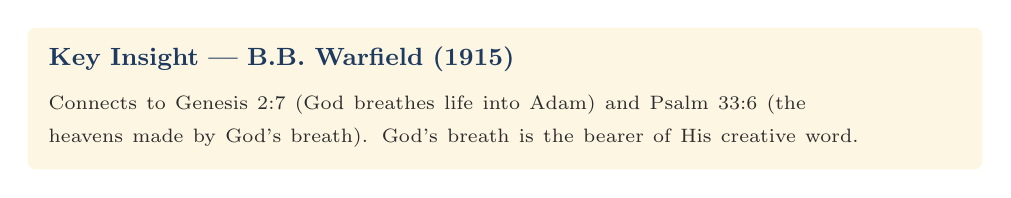
\begin{tikzpicture}
\node[fill=lightgold, rounded corners=3pt, minimum width=\textwidth, minimum height=1.8cm, anchor=north west, text width=0.9\textwidth] at (0,0) {};
\node[anchor=north west, text width=0.85\textwidth] at (0.15,-0.12) {
    {\small\bfseries\color{navy} Key Insight --- B.B.\ Warfield (1915)}\\[4pt]
    {\scriptsize\color{darktext} Connects to Genesis 2:7 (God breathes life into Adam) and Psalm 33:6 (the heavens made by God's breath). God's breath is the bearer of His creative word.}
};
\end{tikzpicture}

\end{column}
\begin{column}{0.48\textwidth}

{\small\bfseries\rmfamily\color{navy} The Four Purposes of Scripture}
\goldline

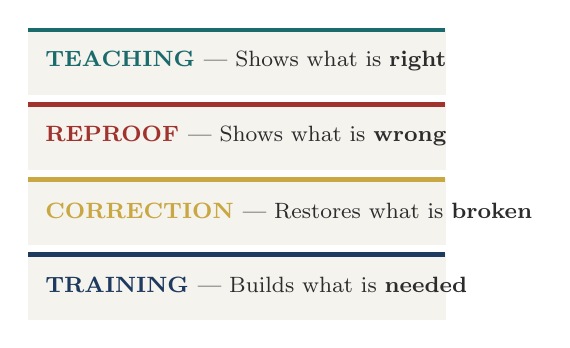
\begin{tikzpicture}[node distance=0.15cm]
\node[fill=offwhite, minimum width=5.3cm, minimum height=0.85cm, anchor=north west] (a) at (0,0) {};
\fill[teal] (0,0) rectangle (5.3,-0.06);
\node[anchor=west] at (0.1,-0.42) {\footnotesize\bfseries\color{teal} TEACHING \normalfont\color{darktext}--- Shows what is \textbf{right}};

\node[fill=offwhite, minimum width=5.3cm, minimum height=0.85cm, anchor=north west] (b) at (0,-0.95) {};
\fill[warmred] (0,-0.95) rectangle (5.3,-1.01);
\node[anchor=west] at (0.1,-1.37) {\footnotesize\bfseries\color{warmred} REPROOF \normalfont\color{darktext}--- Shows what is \textbf{wrong}};

\node[fill=offwhite, minimum width=5.3cm, minimum height=0.85cm, anchor=north west] (c) at (0,-1.9) {};
\fill[gold] (0,-1.9) rectangle (5.3,-1.96);
\node[anchor=west] at (0.1,-2.32) {\footnotesize\bfseries\color{gold} CORRECTION \normalfont\color{darktext}--- Restores what is \textbf{broken}};

\node[fill=offwhite, minimum width=5.3cm, minimum height=0.85cm, anchor=north west] (d) at (0,-2.85) {};
\fill[navy] (0,-2.85) rectangle (5.3,-2.91);
\node[anchor=west] at (0.1,-3.27) {\footnotesize\bfseries\color{navy} TRAINING \normalfont\color{darktext}--- Builds what is \textbf{needed}};
\end{tikzpicture}

\end{column}
\end{columns}

\end{frame}

% ============================================================
% SLIDE 6 — LOGOS VS RHEMA
% ============================================================
\begin{frame}{Logos vs.\ Rhema --- A Balanced View}

\begin{columns}[T]
\begin{column}{0.48\textwidth}
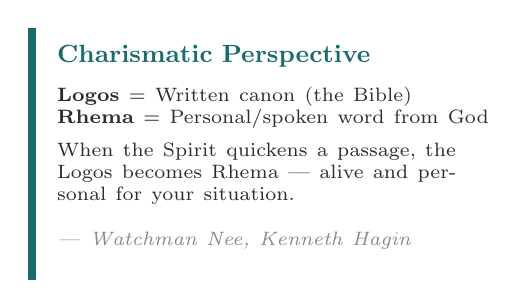
\begin{tikzpicture}
\fill[white] (0,0) rectangle (6,3.2);
\fill[teal] (0,0) rectangle (0.1,3.2);
\node[anchor=north west, text width=5.5cm] at (0.25,3.1) {
    {\small\bfseries\color{teal} Charismatic Perspective}\\[6pt]
    {\scriptsize\color{darktext}
    \textbf{Logos} = Written canon (the Bible)\\
    \textbf{Rhema} = Personal/spoken word from God\\[4pt]
    When the Spirit quickens a passage, the Logos becomes Rhema --- alive and personal for your situation.\\[4pt]
    \textit{\color{softgray}--- Watchman Nee, Kenneth Hagin}}
};
\end{tikzpicture}
\end{column}
\begin{column}{0.48\textwidth}
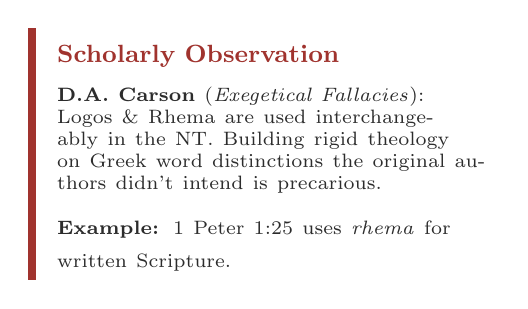
\begin{tikzpicture}
\fill[white] (0,0) rectangle (6,3.2);
\fill[warmred] (0,0) rectangle (0.1,3.2);
\node[anchor=north west, text width=5.5cm] at (0.25,3.1) {
    {\small\bfseries\color{warmred} Scholarly Observation}\\[6pt]
    {\scriptsize\color{darktext}
    \textbf{D.A.\ Carson} (\textit{Exegetical Fallacies}):\\
    Logos \& Rhema are used interchangeably in the NT. Building rigid theology on Greek word distinctions the original authors didn't intend is precarious.\\[4pt]
    \textbf{Example:} 1~Peter 1:25 uses \textit{rhema} for written Scripture.}
};
\end{tikzpicture}
\end{column}
\end{columns}

\vspace{0.2cm}

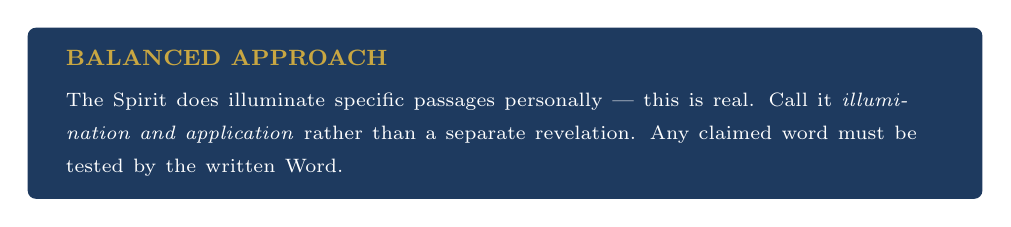
\begin{tikzpicture}
\node[fill=navy, rounded corners=3pt, minimum width=\textwidth, inner sep=8pt, text width=0.92\textwidth] {
    {\footnotesize\bfseries\color{gold} BALANCED APPROACH}\\[3pt]
    {\scriptsize\color{white} The Spirit does illuminate specific passages personally --- this is real. Call it \textit{illumination and application} rather than a separate revelation. Any claimed word must be tested by the written Word.}
};
\end{tikzpicture}

\end{frame}

% ============================================================
% SLIDE 7 — BIBLICAL EXAMPLES (Part 1)
% ============================================================
\begin{frame}{Biblical Examples: Led by the Written Word}

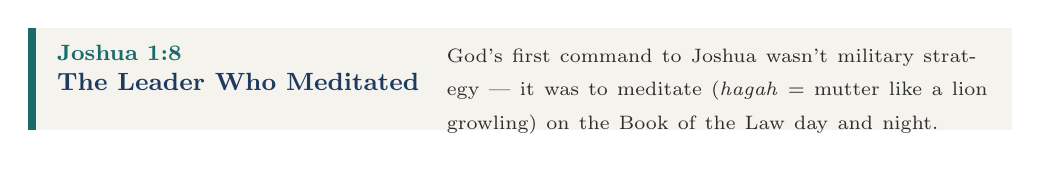
\begin{tikzpicture}
% Example 1
\fill[offwhite] (0,0) rectangle (12.5,1.3);
\fill[teal] (0,0) rectangle (0.1,1.3);
\node[anchor=north west] at (0.25,1.2) {\footnotesize\bfseries\color{teal} Joshua 1:8};
\node[anchor=north west] at (0.25,0.85) {\small\bfseries\rmfamily\color{navy} The Leader Who Meditated};
\node[anchor=north west, text width=7cm] at (5.2,1.15) {\scriptsize\color{darktext} God's first command to Joshua wasn't military strategy --- it was to meditate (\textit{hagah} = mutter like a lion growling) on the Book of the Law day and night.};
\end{tikzpicture}

\vspace{0.15cm}

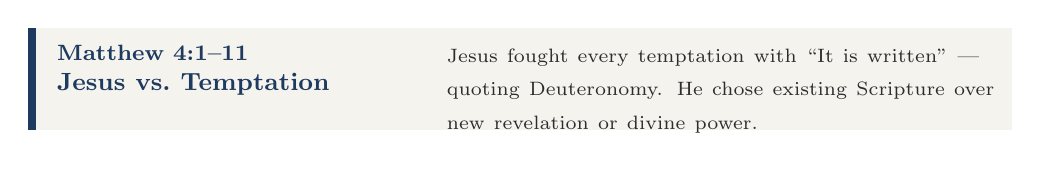
\begin{tikzpicture}
% Example 2
\fill[offwhite] (0,0) rectangle (12.5,1.3);
\fill[navy] (0,0) rectangle (0.1,1.3);
\node[anchor=north west] at (0.25,1.2) {\footnotesize\bfseries\color{navy} Matthew 4:1--11};
\node[anchor=north west] at (0.25,0.85) {\small\bfseries\rmfamily\color{navy} Jesus vs.\ Temptation};
\node[anchor=north west, text width=7cm] at (5.2,1.15) {\scriptsize\color{darktext} Jesus fought every temptation with ``It is written'' --- quoting Deuteronomy. He chose existing Scripture over new revelation or divine power.};
\end{tikzpicture}

\vspace{0.15cm}

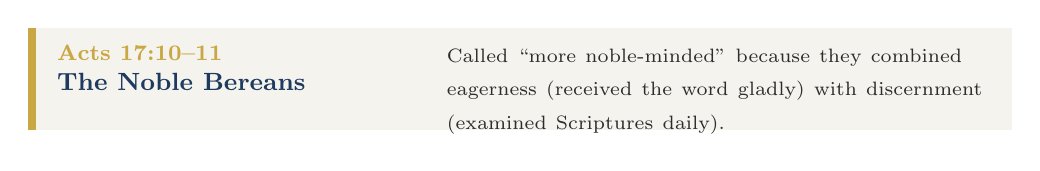
\begin{tikzpicture}
% Example 3
\fill[offwhite] (0,0) rectangle (12.5,1.3);
\fill[gold] (0,0) rectangle (0.1,1.3);
\node[anchor=north west] at (0.25,1.2) {\footnotesize\bfseries\color{gold} Acts 17:10--11};
\node[anchor=north west] at (0.25,0.85) {\small\bfseries\rmfamily\color{navy} The Noble Bereans};
\node[anchor=north west, text width=7cm] at (5.2,1.15) {\scriptsize\color{darktext} Called ``more noble-minded'' because they combined eagerness (received the word gladly) with discernment (examined Scriptures daily).};
\end{tikzpicture}

\end{frame}

% ============================================================
% SLIDE 8 — BIBLICAL EXAMPLES (Part 2)
% ============================================================
\begin{frame}{Biblical Examples (continued)}

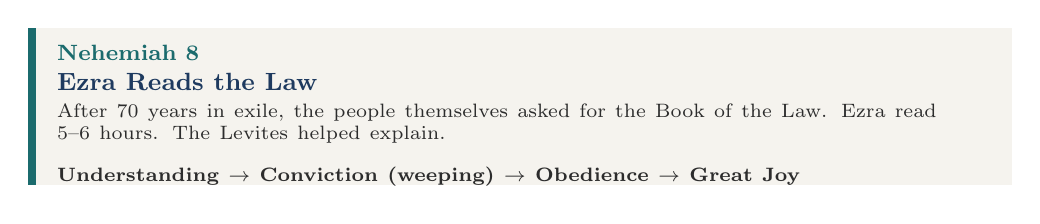
\begin{tikzpicture}
\fill[offwhite] (0,0) rectangle (12.5,2);
\fill[teal] (0,0) rectangle (0.1,2);
\node[anchor=north west] at (0.25,1.9) {\footnotesize\bfseries\color{teal} Nehemiah 8};
\node[anchor=north west] at (0.25,1.55) {\small\bfseries\rmfamily\color{navy} Ezra Reads the Law};
\node[anchor=north west, text width=11.5cm] at (0.25,1.15) {\scriptsize\color{darktext} After 70 years in exile, the people themselves asked for the Book of the Law. Ezra read 5--6 hours. The Levites helped explain.\\[3pt] \textbf{Understanding $\rightarrow$ Conviction (weeping) $\rightarrow$ Obedience $\rightarrow$ Great Joy}};
\end{tikzpicture}

\vspace{0.3cm}

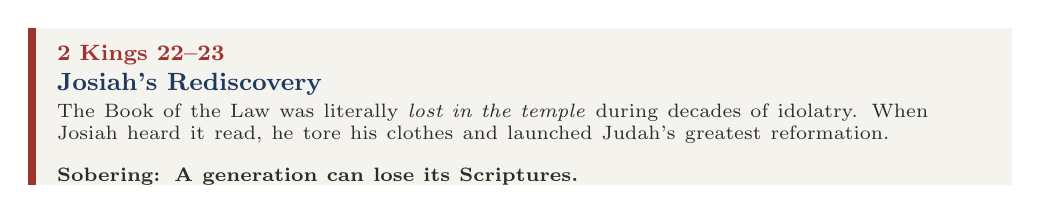
\begin{tikzpicture}
\fill[offwhite] (0,0) rectangle (12.5,2);
\fill[warmred] (0,0) rectangle (0.1,2);
\node[anchor=north west] at (0.25,1.9) {\footnotesize\bfseries\color{warmred} 2 Kings 22--23};
\node[anchor=north west] at (0.25,1.55) {\small\bfseries\rmfamily\color{navy} Josiah's Rediscovery};
\node[anchor=north west, text width=11.5cm] at (0.25,1.15) {\scriptsize\color{darktext} The Book of the Law was literally \textit{lost in the temple} during decades of idolatry. When Josiah heard it read, he tore his clothes and launched Judah's greatest reformation.\\[3pt] \textbf{Sobering: A generation can lose its Scriptures.}};
\end{tikzpicture}

\end{frame}

% ============================================================
% SLIDE 9 — POWER OF 4
% ============================================================
{
\setbeamercolor{background canvas}{bg=navy}
\begin{frame}[plain]
\darkfooteroverlay
\vspace{0.3cm}
{\Large\bfseries\rmfamily\color{white} The ``Power of 4'' --- Research You Need to Know}\\[2pt]
{\color{gold}\rule{3cm}{1.5pt}}

\vspace{0.3cm}

\begin{columns}[T]
\begin{column}{0.38\textwidth}
{\fontsize{36}{40}\selectfont\bfseries\rmfamily\color{gold} 100,000+}\\[4pt]
{\small\color{softgray} people surveyed over 8 years\\(Center for Bible Engagement)}
\end{column}
\begin{column}{0.58\textwidth}
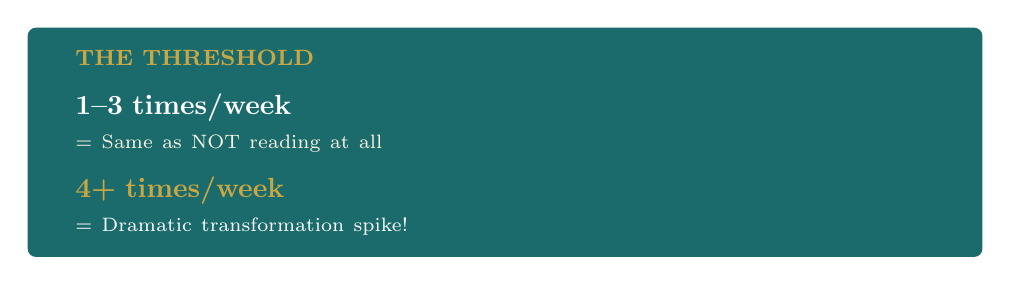
\begin{tikzpicture}
\node[fill=teal, rounded corners=3pt, minimum width=\textwidth, inner sep=8pt, text width=0.9\textwidth] {
    {\footnotesize\bfseries\color{gold} THE THRESHOLD}\\[6pt]
    {\normalsize\bfseries\color{white} 1--3 times/week}\\
    {\scriptsize\color{lightgold} = Same as NOT reading at all}\\[6pt]
    {\normalsize\bfseries\color{gold} 4+ times/week}\\
    {\scriptsize\color{white} = Dramatic transformation spike!}
};
\end{tikzpicture}
\end{column}
\end{columns}

\vspace{0.3cm}

\begin{columns}[T]
\begin{column}{0.48\textwidth}

\begin{tikzpicture}
\node[fill=deepnavy, rounded corners=3pt, minimum width=\textwidth, inner sep=8pt, text width=0.85\textwidth] {
    {\footnotesize\bfseries\color{warmred} LOWER at 4+/week}\\[4pt]
    {\scriptsize\color{white} Drinking to excess, pornography, lashing out in anger, gossiping, lying, gambling}
};
\end{tikzpicture}
\end{column}
\begin{column}{0.48\textwidth}

\begin{tikzpicture}
\node[fill=deepnavy, rounded corners=3pt, minimum width=\textwidth, inner sep=8pt, text width=0.85\textwidth] {
    {\footnotesize\bfseries\color{gold} HIGHER at 4+/week}\\[4pt]
    {\scriptsize\color{white} Faith-sharing, spiritual growth, moral decision-making, resilience, proactive service}
};
\end{tikzpicture}
\end{column}
\end{columns}

\end{frame}
}

% ============================================================
% SLIDE 10 — DISCUSSION QUESTIONS
% ============================================================
\begin{frame}{Discussion Questions}

\begin{columns}[T]
\begin{column}{0.48\textwidth}
{\small\bfseries\color{teal} KEY UNDERTONE QUESTIONS}\\[6pt]
{\small
\textbf{\color{navy}1.}~If Scripture is sufficient, why do believers still struggle with direction?\\[5pt]
\textbf{\color{navy}2.}~What does it mean \textit{practically} that Scripture is God-breathed?\\[5pt]
\textbf{\color{navy}3.}~The Bereans searched daily. What would that look like for you?\\[5pt]
\textbf{\color{navy}4.}~What prevents you from crossing the 4~times/week threshold?
}
\end{column}
\begin{column}{0.48\textwidth}
{\small\bfseries\color{warmred} CONTRASTING QUESTIONS}\\[6pt]
{\small
\textbf{\color{navy}1.}~Can the written Word become a personal Rhema word? How?\\[5pt]
\textbf{\color{navy}2.}~Is reading enough, or must the Spirit always accompany?\\[5pt]
\textbf{\color{navy}3.}~How do we avoid bibliolatry while honoring Scripture's authority?\\[5pt]
\textbf{\color{navy}4.}~Is it possible to know the Bible intellectually but miss its power?
}
\end{column}
\end{columns}

\end{frame}

% ============================================================
% SLIDE 11 — QUOTES
% ============================================================
{
\setbeamercolor{background canvas}{bg=navy}
\begin{frame}[plain]
\darkfooteroverlay
\vspace{0.3cm}
{\Large\bfseries\rmfamily\color{white} Voices Across the Ages}\\[2pt]
{\color{gold}\rule{3cm}{1.5pt}}

\vspace{0.3cm}

\begin{tikzpicture}
\foreach \txt/\auth/\ypos in {%
    {``The Bible is alive, it speaks to me; it has feet, it runs after me; it has hands, it lays hold of me.''}/{--- Martin Luther}/0,%
    {``Oh, give me that book! At any price, give me the book of God!''}/{--- John Wesley}/-1.0,%
    {``Nobody ever outgrows Scripture; the Book widens and deepens with our years.''}/{--- Charles Spurgeon}/-2.0,%
    {``Whatever keeps me from my Bible is my enemy, however harmless it may appear.''}/{--- A.W.\ Tozer}/-3.0,%
    {``I like to read mine in the Holy Ghost.''}/{--- Smith Wigglesworth (Pentecostal pioneer)}/-4.0%
}{
    \fill[gold] (0,\ypos) rectangle (0.06,\ypos-0.7);
    \node[anchor=north west, text width=11.5cm] at (0.2,\ypos-0.05) {\scriptsize\color{white}\rmfamily\itshape \txt};
    \node[anchor=north west] at (0.2,\ypos-0.55) {\tiny\color{gold} \auth};
}
\end{tikzpicture}

\end{frame}
}

% ============================================================
% SLIDE 12 — TAKE-HOME TASKS
% ============================================================
\begin{frame}{Take-Home Tasks This Week}

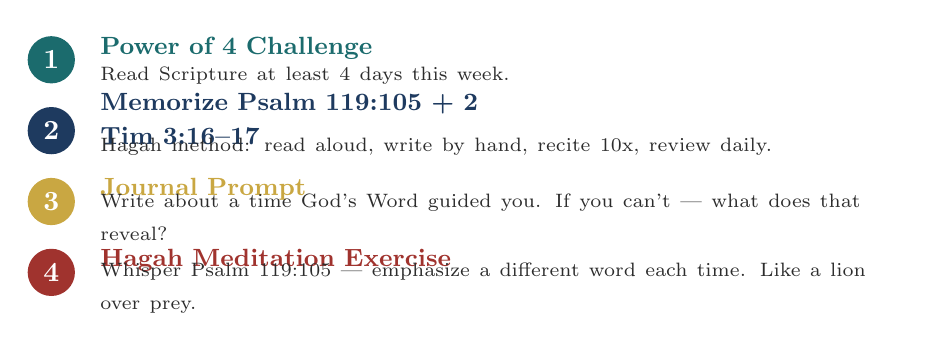
\begin{tikzpicture}
% Task 1
\fill[teal] (0,0) circle (0.3);
\node[white,font=\bfseries\rmfamily] at (0,0) {1};
\node[anchor=west, text width=5cm] at (0.5,0.15) {\small\bfseries\color{teal} Power of 4 Challenge};
\node[anchor=west, text width=10cm] at (0.5,-0.2) {\scriptsize\color{darktext} Read Scripture at least 4 days this week.};

% Task 2
\fill[navy] (0,-0.9) circle (0.3);
\node[white,font=\bfseries\rmfamily] at (0,-0.9) {2};
\node[anchor=west, text width=5cm] at (0.5,-0.75) {\small\bfseries\color{navy} Memorize Psalm 119:105 + 2 Tim 3:16--17};
\node[anchor=west, text width=10cm] at (0.5,-1.1) {\scriptsize\color{darktext} Hagah method: read aloud, write by hand, recite 10x, review daily.};

% Task 3
\fill[gold] (0,-1.8) circle (0.3);
\node[white,font=\bfseries\rmfamily] at (0,-1.8) {3};
\node[anchor=west, text width=5cm] at (0.5,-1.65) {\small\bfseries\color{gold} Journal Prompt};
\node[anchor=west, text width=10cm] at (0.5,-2.0) {\scriptsize\color{darktext} Write about a time God's Word guided you. If you can't --- what does that reveal?};

% Task 4
\fill[warmred] (0,-2.7) circle (0.3);
\node[white,font=\bfseries\rmfamily] at (0,-2.7) {4};
\node[anchor=west, text width=5cm] at (0.5,-2.55) {\small\bfseries\color{warmred} Hagah Meditation Exercise};
\node[anchor=west, text width=10cm] at (0.5,-2.9) {\scriptsize\color{darktext} Whisper Psalm 119:105 --- emphasize a different word each time. Like a lion over prey.};
\end{tikzpicture}

\end{frame}

% ============================================================
% SLIDE 13 — CONCLUSION / GUARDRAIL
% ============================================================
{
\setbeamercolor{background canvas}{bg=navy}
\begin{frame}[plain]
\darkfooteroverlay
\vspace{0.3cm}
{\Large\bfseries\rmfamily\color{white} The Written Word Comes First}\\[2pt]
{\color{gold}\rule{3cm}{1.5pt}}

\vspace{0.25cm}

{\small\itshape\color{white} In every biblical example, the pattern is the same:}\\[6pt]

{\small\color{white}
$\rightarrow$~Joshua needed the Book of the Law before battle.\\[3pt]
$\rightarrow$~Jesus used ``It is written'' before new revelation.\\[3pt]
$\rightarrow$~The Bereans tested spoken teaching against Scripture.\\[3pt]
$\rightarrow$~Ezra read the Torah --- revival broke out.\\[3pt]
$\rightarrow$~Josiah found the Law --- reformation followed.
}

\vspace{0.4cm}

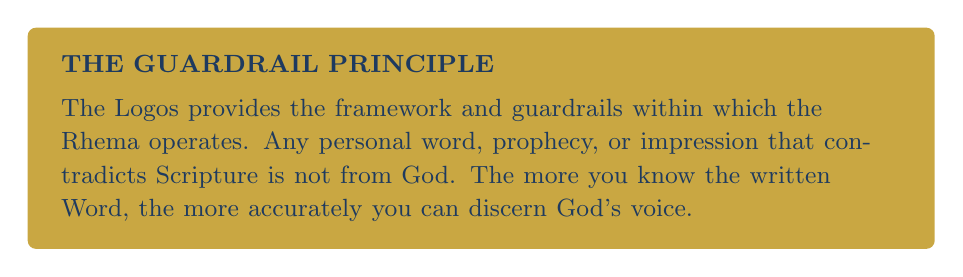
\begin{tikzpicture}
\node[fill=gold, rounded corners=3pt, minimum width=0.95\textwidth, inner sep=10pt, text width=0.88\textwidth] {
    {\small\bfseries\color{navy} THE GUARDRAIL PRINCIPLE}\\[4pt]
    {\small\color{navy} The Logos provides the framework and guardrails within which the Rhema operates. Any personal word, prophecy, or impression that contradicts Scripture is not from God. The more you know the written Word, the more accurately you can discern God's voice.}
};
\end{tikzpicture}

\end{frame}
}

% ============================================================
% SLIDE 14 — CLOSING
% ============================================================
{
\setbeamercolor{background canvas}{bg=navy}
\begin{frame}[plain]
\darkfooteroverlay
\vfill
\begin{center}

{\Large\rmfamily\itshape\color{white} ``Open my eyes, that I may behold\\wondrous things out of your law.''}\\[6pt]
{\normalsize\color{gold} --- Psalm 119:18}

\vspace{0.25cm}
{\color{gold}\rule{4cm}{1.5pt}}
\vspace{0.3cm}

{\small\bfseries\color{gold} NEXT SESSION}\\[4pt]
{\Large\bfseries\rmfamily\color{white} Living by the Spoken Word (\textit{Rhema})}\\[6pt]
{\normalsize\color{gold} Matthew 4:4~~$\cdot$~~John 6:63}\\[4pt]
{\small\color{softgray} March 27, 2026}

\vspace{0.4cm}

{\small\itshape\color{white} How does God make the written Word come alive personally?\\How does a verse you've read a hundred times suddenly pierce\\your heart at the exact right moment?}

\vspace{0.3cm}

{\normalsize\color{gold}\textsc{ICF Word Study} --- \textit{Moscow Good News Church}}\\[4pt]
{\normalsize\color{white}\itshape $\sim$~Roger Nick Anaedevha}

\end{center}
\vfill
\end{frame}
}

\end{document}
